\documentclass[letterpaper,11pt]{article}

\usepackage{geometry}
\usepackage{pslatex}
\usepackage{fancyhdr}
\usepackage{graphicx}
\usepackage{color}
\usepackage{tikz}
\usepackage{setspace}
\geometry{ margin = 1.0in }

\pagestyle{fancy}
\lhead{{\bf Lecture 31}}
\chead{{\bf CMPSC 465 Fall 2020}}
\rhead{{\bf Mingfu Shao}}

\setlength\parindent{0em}
\setlength\parskip{8pt}
%\setlength{\fboxsep}{6pt}

\usepackage{amsthm}
\newtheoremstyle{mytheorem}
  {\parskip} % Space above
  {0em} % Space below
  {} % Body font
  {} % Indent amount
  {\bfseries} % Theorem head font
  {.} % Punctuation after theorem head
  {.5em} % Space after theorem head
  {} % Theorem head spec (can be left empty, meaning `normal')

\theoremstyle{mytheorem}
\newtheorem{definition}{Definition}
\newtheorem{property}{Property}
\newtheorem{claim}{Claim}
\newtheorem{fact}{Fact}
\newtheorem{corollary}{Corollary}

% for algorithms
\newcommand{\aaa}[1]{\hspace{0.65cm}\parbox[t]{15.3cm}{#1}}
\newcommand{\aab}[1]{\hspace{1.15cm}\parbox[t]{15.0cm}{#1}}
\newcommand{\aac}[1]{\hspace{1.65cm}\parbox[t]{15.0cm}{#1}}
\newcommand{\aad}[1]{\hspace{2.15cm}\parbox[t]{15.0cm}{#1}}
\newcommand{\aae}[1]{\hspace{2.65cm}\parbox[t]{15.0cm}{#1}}
\newcommand{\aaf}[1]{\hspace{3.15cm}\parbox[t]{15.0cm}{#1}}
\newcommand{\aaA}[2]{\hspace{0.5cm} {\tikz[overlay] \draw (0.1, -0.1) -- (0.1, #1 * -1.5em + 0.6em);} \parbox[t]{15.0cm}{#2}}
\newcommand{\aaB}[2]{\hspace{1.0cm} {\tikz[overlay] \draw (0.1, -0.1) -- (0.1, #1 * -1.5em + 0.6em);} \parbox[t]{15.0cm}{#2}}
\newcommand{\aaC}[2]{\hspace{1.5cm} {\tikz[overlay] \draw (0.1, -0.1) -- (0.1, #1 * -1.5em + 0.6em);} \parbox[t]{15.0cm}{#2}}
\newcommand{\aaD}[2]{\hspace{2.0cm} {\tikz[overlay] \draw (0.1, -0.1) -- (0.1, #1 * -1.5em + 0.6em);} \parbox[t]{15.0cm}{#2}}
\newcommand{\aaE}[2]{\hspace{2.5cm} {\tikz[overlay] \draw (0.1, -0.1) -- (0.1, #1 * -1.5em + 0.6em);} \parbox[t]{15.0cm}{#2}}
\newcommand{\xxx}{\par\vspace{0.1cm}}

\begin{document}

\section*{Minimum Spanning Tree~(Continued)}

\subsection*{The Cut Property}

The cut-property describes how to \emph{augment a partial MST}, 
formally described below.
A \emph{partial} MST is a subset of edges of a MST~(see Figure~\ref{fig:spanning}).
This property gives a way to iteratively construct a MST: one can iteratively
apply it to augment a partial MST~(intially empty) until it becomes a (complete) 
MST~(i.e., its size becomes $|V| - 1$).
In fact, both Kruskal's algorithm and Prim's algorithm
are essentially using this property.
Their correctness therefore can be proved with this property too.

\begin{claim}[Cut-Property]
Let $E_1$ be a partial MST of graph $G = (V, E)$. %.
Let $C = (S,V\setminus S)$ be a cut of $G$.
If $E(C) \cap E_1 = \emptyset$, %~(i.e., the cut-edges w.r.t.\ $C$ doesn't overlap with $E_1$
then $E_1\cup \{e^*\}$ is also a partial MST, where $e^* := \arg\min_{e\in E(C)} w(e)$.
\end{claim}

In other words, suppose you have a partial solution $E_1$ that you know
are part of a MST~(i.e., there exists a MST $T^* = (V, E^*)$ such that $E_1\subset E^*$). 
In order to augment $E_1$, you will need to find a cut $C = (S, V\setminus S)$ of $G$.
If the cut-edges w.r.t.\ $C$ doesn't overlap with $E_1$~(i.e., $E(C)\cap E_1 = \emptyset$),
then the smallest cut-edge, i.e., $e^* := \arg\min_{e\in E(C)} w(e)$,
can be safely included.

\begin{figure}[h]
\centering{

\tikzset{every picture/.style={line width=0.75pt}} %set default line width to 0.75pt        

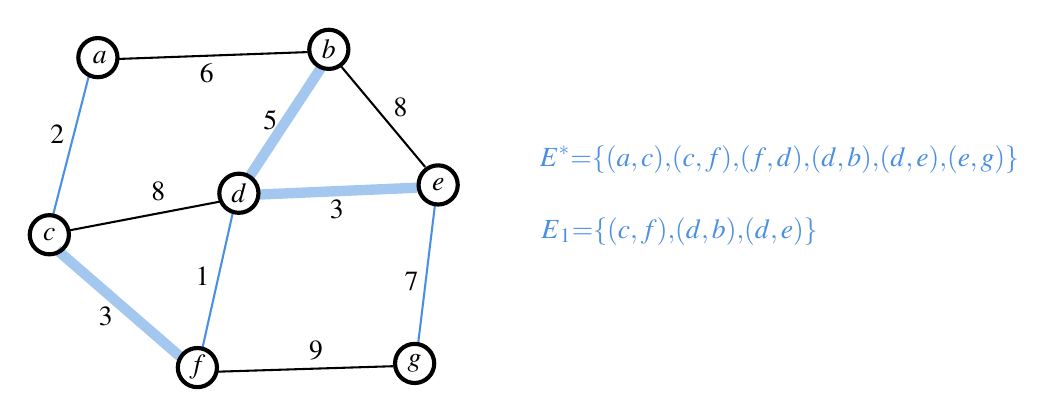
\begin{tikzpicture}[x=0.5pt,y=0.5pt,yscale=-1,xscale=1]
%uncomment if require: \path (0,294); %set diagram left start at 0, and has height of 294

%Straight Lines [id:da823970354045778] 
\draw [color={rgb, 255:red, 0; green, 0; blue, 0 }  ,draw opacity=1 ][line width=0.75]    (237,42) -- (298,115) ;
%Straight Lines [id:da271237396517352] 
\draw [color={rgb, 255:red, 0; green, 0; blue, 0 }  ,draw opacity=1 ][line width=0.75]    (147,263) -- (275,259) ;
%Straight Lines [id:da6657573604931601] 
\draw [color={rgb, 255:red, 74; green, 144; blue, 226 }  ,draw opacity=0.5 ][line width=3.75]    (32,175) -- (122,253) ;
%Straight Lines [id:da31661075744879486] 
\draw [color={rgb, 255:red, 0; green, 0; blue, 0 }  ,draw opacity=1 ][line width=0.75]    (40,161) -- (150,140) ;
%Straight Lines [id:da9969849240959807] 
\draw [color={rgb, 255:red, 74; green, 144; blue, 226 }  ,draw opacity=1 ][line width=0.75]    (55,49) -- (29,150) ;
%Straight Lines [id:da14506071047898028] 
\draw [color={rgb, 255:red, 0; green, 0; blue, 0 }  ,draw opacity=1 ][line width=0.75]    (75,37) -- (213,32) ;
%Straight Lines [id:da8946288202546534] 
\draw [color={rgb, 255:red, 74; green, 144; blue, 226 }  ,draw opacity=0.5 ][line width=3.75]    (223,43) -- (171,122) ;
%Straight Lines [id:da15496081521651384] 
\draw [color={rgb, 255:red, 74; green, 144; blue, 226 }  ,draw opacity=1 ][line width=0.75]    (159,148) -- (137,246) ;
%Straight Lines [id:da2163317830574415] 
\draw [color={rgb, 255:red, 74; green, 144; blue, 226 }  ,draw opacity=1 ][line width=0.75]    (305,143) -- (293,242) ;
%Straight Lines [id:da5391246746067021] 
\draw [color={rgb, 255:red, 74; green, 144; blue, 226 }  ,draw opacity=0.5 ][line width=3.75]    (292,130) -- (177,135) ;

% Text Node
\draw  [line width=1.5]   (307.38, 128) circle [x radius= 14.15, y radius= 14.15]   ;
\draw (307.38,128) node   [align=left] {$\displaystyle e$};
% Text Node
\draw  [line width=1.5]   (61.48, 36) circle [x radius= 14.15, y radius= 14.15]   ;
\draw (55.98,36) node [anchor=west] [inner sep=0.75pt]   [align=left] {$\displaystyle a$};
% Text Node
\draw  [line width=1.5]   (228.38, 30) circle [x radius= 14.15, y radius= 14.15]   ;
\draw (228.38,30) node   [align=left] {$\displaystyle b$};
% Text Node
\draw  [line width=1.5]   (26.38, 164) circle [x radius= 14.15, y radius= 14.15]   ;
\draw (26.38,164) node   [align=left] {$\displaystyle c$};
% Text Node
\draw  [line width=1.5]   (163.38, 134) circle [x radius= 14.15, y radius= 14.15]   ;
\draw (163.38,134) node   [align=left] {$\displaystyle d$};
% Text Node
\draw  [line width=1.5]   (133.38, 260) circle [x radius= 14.15, y radius= 14.15]   ;
\draw (133.38,260) node   [align=left] {$\displaystyle f$};
% Text Node
\draw  [line width=1.5]   (290.38, 257) circle [x radius= 14.15, y radius= 14.15]   ;
\draw (290.38,257) node   [align=left] {$\displaystyle g$};
% Text Node
\draw (25.24,83.06) node [anchor=north west][inner sep=0.75pt]   [align=left] {$\displaystyle 2$};
% Text Node
\draw (133.24,38.06) node [anchor=north west][inner sep=0.75pt]   [align=left] {$\displaystyle 6$};
% Text Node
\draw (227.24,137.06) node [anchor=north west][inner sep=0.75pt]   [align=left] {$\displaystyle 3$};
% Text Node
\draw (179.24,72.06) node [anchor=north west][inner sep=0.75pt]   [align=left] {$\displaystyle 5$};
% Text Node
\draw (98.24,124.06) node [anchor=north west][inner sep=0.75pt]   [align=left] {$\displaystyle 8$};
% Text Node
\draw (60.24,214.06) node [anchor=north west][inner sep=0.75pt]   [align=left] {$\displaystyle 3$};
% Text Node
\draw (130.24,185.06) node [anchor=north west][inner sep=0.75pt]   [align=left] {$\displaystyle 1$};
% Text Node
\draw (273.24,63.06) node [anchor=north west][inner sep=0.75pt]   [align=left] {$\displaystyle 8$};
% Text Node
\draw (212.24,239.06) node [anchor=north west][inner sep=0.75pt]   [align=left] {$\displaystyle 9$};
% Text Node
\draw (281.24,189) node [anchor=north west][inner sep=0.75pt]   [align=left] {$\displaystyle 7$};
% Text Node
\draw (379,98) node [anchor=north west][inner sep=0.75pt]   [align=left] {$\displaystyle \textcolor[rgb]{0.29,0.56,0.89}{E}\textcolor[rgb]{0.29,0.56,0.89}{^{*}}\textcolor[rgb]{0.29,0.56,0.89}{=}\textcolor[rgb]{0.29,0.56,0.89}{\{}\textcolor[rgb]{0.29,0.56,0.89}{(}\textcolor[rgb]{0.29,0.56,0.89}{a,c}\textcolor[rgb]{0.29,0.56,0.89}{)}\textcolor[rgb]{0.29,0.56,0.89}{,}\textcolor[rgb]{0.29,0.56,0.89}{(}\textcolor[rgb]{0.29,0.56,0.89}{c,f}\textcolor[rgb]{0.29,0.56,0.89}{)}\textcolor[rgb]{0.29,0.56,0.89}{,}\textcolor[rgb]{0.29,0.56,0.89}{(}\textcolor[rgb]{0.29,0.56,0.89}{f,d}\textcolor[rgb]{0.29,0.56,0.89}{)}\textcolor[rgb]{0.29,0.56,0.89}{,}\textcolor[rgb]{0.29,0.56,0.89}{(}\textcolor[rgb]{0.29,0.56,0.89}{d,b}\textcolor[rgb]{0.29,0.56,0.89}{)}\textcolor[rgb]{0.29,0.56,0.89}{,}\textcolor[rgb]{0.29,0.56,0.89}{(}\textcolor[rgb]{0.29,0.56,0.89}{d,e}\textcolor[rgb]{0.29,0.56,0.89}{)}\textcolor[rgb]{0.29,0.56,0.89}{,}\textcolor[rgb]{0.29,0.56,0.89}{(}\textcolor[rgb]{0.29,0.56,0.89}{e,g}\textcolor[rgb]{0.29,0.56,0.89}{)}\textcolor[rgb]{0.29,0.56,0.89}{\}}$};
% Text Node
\draw (380,150) node [anchor=north west][inner sep=0.75pt]   [align=left] {$\displaystyle \textcolor[rgb]{0.29,0.56,0.89}{E}\textcolor[rgb]{0.29,0.56,0.89}{_{1}}\textcolor[rgb]{0.29,0.56,0.89}{=}\textcolor[rgb]{0.29,0.56,0.89}{\{}\textcolor[rgb]{0.29,0.56,0.89}{(}\textcolor[rgb]{0.29,0.56,0.89}{c,f}\textcolor[rgb]{0.29,0.56,0.89}{)}\textcolor[rgb]{0.29,0.56,0.89}{,}\textcolor[rgb]{0.29,0.56,0.89}{(}\textcolor[rgb]{0.29,0.56,0.89}{d,b}\textcolor[rgb]{0.29,0.56,0.89}{)}\textcolor[rgb]{0.29,0.56,0.89}{,}\textcolor[rgb]{0.29,0.56,0.89}{(}\textcolor[rgb]{0.29,0.56,0.89}{d,e}\textcolor[rgb]{0.29,0.56,0.89}{)}\textcolor[rgb]{0.29,0.56,0.89}{\}}$};


\end{tikzpicture}

}
\caption{Illustrating the cut-property.}
\label{fig:spanning}
\end{figure}

See above example. The blue edges~(including thin and thick ones)
gives a MST $E^*$, and the thick ones, denoted as $E_1$, represents a partial MST.
Try following cuts $C = (S, V\setminus S)$ where $S$ is specified:
\vspace*{-\topsep}
\begin{enumerate}
\item $S = \{a\}$. $E(C) = \{(a,c), (a,b)\}$. $E(C) \cap E_1 = \emptyset$. $e^* = (a,c)$.
So $E_1\cup\{e^*\}$ is a partial MST.
\item $S = \{a,c,f\}$. $E(C) = \{(a,b), (c,d), (f,d), (f,g)\}$. $E(C) \cap E_1 = \emptyset$. $e^* = (d,f)$.
So $E_1\cup\{e^*\}$ is a partial MST.
\item $S = \{a,g\}$. $E(C) = \{(a,b), (a,c), (f,g), (e,g)\}$. $E(C) \cap E_1 = \emptyset$. $e^* = (a,c)$.
So $E_1\cup\{e^*\}$ is a partial MST.
\item $S = \{a,c\}$. $E(C) = \{(a,b), (c,d), (c,f)\}$. $E(C) \cap E_1 = \{(c,f)\}$. So we can't get a larger partial MST with this cut.
\end{enumerate}

Note that, a partial MST $E_1$ partitions all vertices of $G$ into disjoint connected components.
(Like in above example there are 4 components: $\{a\}, \{c,f\}, \{b,d,e\}, \{g\}$, formed by $E_1$.)
Clearly, a cut $C=\{S,V\setminus S\}$ satisfies $E(C) \cap E_1 = \emptyset$ if and only if for each component
either $S$ includes it entirely or excludes it entirely;
in other words in order not to overlap with $E_1$, a cut just needs to avoid ``breaking''
any connected components formed by $E_1$.

We now prove above claim.  See Figure~\ref{fig:proof}.
The setup is a MST $E^*$, a partial MST $E_1\subset E^*$,
and a cut $C = (S,V\setminus S)$ satisfying that $E(C)\cap E_1 = \emptyset$.
And we need to prove that $E_1\cup \{e^*\}$ is a (partial) MST too,
where $e^*$ is the smallest cut-edge w.r.t.\ $C$.

Consider two cases. If $e^* \in E^*$,
(in Figure~\ref{fig:proof}, this means $e^*$ is one of $\{(a,c),(c,d),(d,f),(d,e)\}$),
then obvisously in this case $E_1\cup \{e^*\}$ is a (partial) MST, and this MST is $E^*$.
This is a trivial case.

The second case is that $e^* \not\in E^*$.
(In Figure~\ref{fig:proof}, this means $e^*$ is one of $\{(b,e),(b,h)\}$.)
Assume that $e^* = (u,v)$ where $u\in S$ and $v\notin S$.
(In Figure~\ref{fig:proof}, w.l.o.g., we assume $e^* = (b,h)$, i.e., $u= b$ and $v=h$.)
Since $E^*$ is a spanning tree, there exists a unique path $p$ from $u$ to $v$ using edges in $E^*$.
(In Figure~\ref{fig:proof}, path $p$ is $(b,a)\to(a,c)\to(c,d)\to(d,e)\to(e,i)\to(i,h)$.)
Since $u\in S$ and $v\notin S$, path $p$ must ``cross'' cut $C$, i.e., 
we must have that edges of $p$ overlaps with cut-edges: $p\cap E(C)\neq \emptyset$.
(In Figure~\ref{fig:proof}, $p\cap E(C) = \{(a,c),(c,d),(d,e)\}$.)
Pick an arbitrary edge $e'$ from $p\cap E(C)$ and build
$E'$ by replacing $e'$ with $e^*$, i.e., $E' = E^* \setminus \{e'\} \cup \{e^*\}$.
(In Figure~\ref{fig:proof}, we can pick $e' = (a,c)$ and build $E' = \{(a,b),(c,d),(d,f),(d,e),(e,g),(e,i),(h,i),(b,h)\}$.)
We can show that $E'$ is still a spanning tree of $G$, as $|E'| = |E^*|$ and it connects all vertices~(removing $e'$ breaks
all vertices into 2 components where $u$ and $v$ are separated into different components, but adding $e^* = (u,v)$ glues them together).
How about the total weight of $E'$? Clearly, $w(E') = w(E^*) - w(e') + w(e^*)$.
Since $e^*$ is the smallest cut-edge and $e'$ is one of the cut-edges, we have $w(e') \ge w(e^*)$.
This gives $w(E') \le w(E^*)$. As $E^*$ is a MST, we must have that $E'$ is a MST too.
As now both $E_1$ and $e^*$ are in $E'$, we conclude that $E_1\cup \{e^*\}$ is a partial MST~(and the MST is $E'$). \qed

\begin{figure}[h]
\centering{

\tikzset{every picture/.style={line width=0.75pt}} %set default line width to 0.75pt        

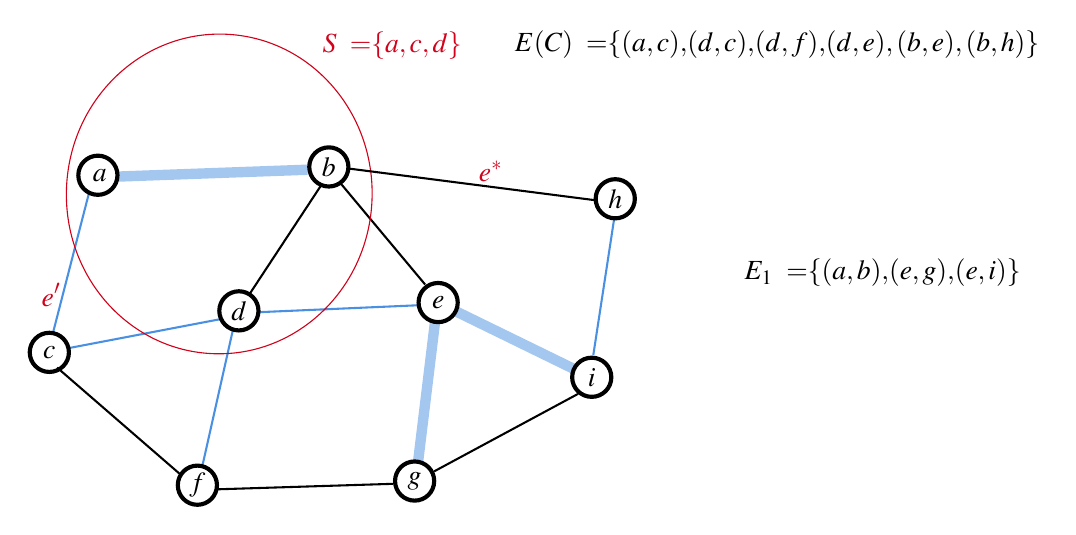
\begin{tikzpicture}[x=0.5pt,y=0.5pt,yscale=-1,xscale=1]
%uncomment if require: \path (0,388); %set diagram left start at 0, and has height of 388

%Straight Lines [id:da6859712806144006] 
\draw [color={rgb, 255:red, 0; green, 0; blue, 0 }  ,draw opacity=1 ][line width=0.75]    (232,125) -- (293,198) ;
%Straight Lines [id:da43828905709564314] 
\draw [color={rgb, 255:red, 0; green, 0; blue, 0 }  ,draw opacity=1 ][line width=0.75]    (142,346) -- (270,342) ;
%Straight Lines [id:da6385368954330931] 
\draw [color={rgb, 255:red, 0; green, 0; blue, 0 }  ,draw opacity=1 ][line width=0.75]    (27,258) -- (117,336) ;
%Straight Lines [id:da061278223687582845] 
\draw [color={rgb, 255:red, 74; green, 144; blue, 226 }  ,draw opacity=1 ][line width=0.75]    (35,244) -- (145,223) ;
%Straight Lines [id:da125058897644165] 
\draw [color={rgb, 255:red, 74; green, 144; blue, 226 }  ,draw opacity=1 ][line width=0.75]    (50,132) -- (24,233) ;
%Straight Lines [id:da7561477389708726] 
\draw [color={rgb, 255:red, 74; green, 144; blue, 226 }  ,draw opacity=0.5 ][line width=3.75]    (70,120) -- (208,115) ;
%Straight Lines [id:da8045438090716241] 
\draw [color={rgb, 255:red, 0; green, 0; blue, 0 }  ,draw opacity=1 ][line width=0.75]    (218,126) -- (166,205) ;
%Straight Lines [id:da7384444755679203] 
\draw [color={rgb, 255:red, 74; green, 144; blue, 226 }  ,draw opacity=1 ][line width=0.75]    (154,231) -- (132,329) ;
%Straight Lines [id:da7781378597799559] 
\draw [color={rgb, 255:red, 74; green, 144; blue, 226 }  ,draw opacity=0.5 ][line width=3.75]    (300,226) -- (288,325) ;
%Straight Lines [id:da6283012441188964] 
\draw [color={rgb, 255:red, 74; green, 144; blue, 226 }  ,draw opacity=1 ][line width=0.75]    (287,213) -- (172,218) ;
%Shape: Ellipse [id:dp6140347486409217] 
\draw  [color={rgb, 255:red, 208; green, 2; blue, 27 }  ,draw opacity=1 ] (33.78,128.41) .. controls (36.15,64.65) and (87.51,14.79) .. (148.48,17.06) .. controls (209.45,19.33) and (256.96,72.86) .. (254.59,136.62) .. controls (252.22,200.38) and (200.87,250.23) .. (139.89,247.96) .. controls (78.92,245.7) and (31.41,192.17) .. (33.78,128.41) -- cycle ;
%Straight Lines [id:da9156710101046748] 
\draw [color={rgb, 255:red, 0; green, 0; blue, 0 }  ,draw opacity=1 ][line width=0.75]    (236.5,114) -- (415.5,137) ;
%Straight Lines [id:da2929261017329614] 
\draw [color={rgb, 255:red, 74; green, 144; blue, 226 }  ,draw opacity=1 ][line width=0.75]    (414.5,249) -- (429.5,151) ;
%Straight Lines [id:da47669871576284994] 
\draw [color={rgb, 255:red, 74; green, 144; blue, 226 }  ,draw opacity=0.5 ][line width=3.75]    (314.5,217) -- (400.5,259) ;
%Straight Lines [id:da851369784287132] 
\draw [color={rgb, 255:red, 0; green, 0; blue, 0 }  ,draw opacity=1 ][line width=0.75]    (299.5,333) -- (403.5,277) ;

% Text Node
\draw  [line width=1.5]   (302.38, 211) circle [x radius= 14.15, y radius= 14.15]   ;
\draw (302.38,211) node   [align=left] {$\displaystyle e$};
% Text Node
\draw  [line width=1.5]   (56.48, 119) circle [x radius= 14.15, y radius= 14.15]   ;
\draw (50.98,119) node [anchor=west] [inner sep=0.75pt]   [align=left] {$\displaystyle a$};
% Text Node
\draw  [line width=1.5]   (223.38, 113) circle [x radius= 14.15, y radius= 14.15]   ;
\draw (223.38,113) node   [align=left] {$\displaystyle b$};
% Text Node
\draw  [line width=1.5]   (21.38, 247) circle [x radius= 14.15, y radius= 14.15]   ;
\draw (21.38,247) node   [align=left] {$\displaystyle c$};
% Text Node
\draw  [line width=1.5]   (158.38, 217) circle [x radius= 14.15, y radius= 14.15]   ;
\draw (158.38,217) node   [align=left] {$\displaystyle d$};
% Text Node
\draw  [line width=1.5]   (128.38, 343) circle [x radius= 14.15, y radius= 14.15]   ;
\draw (128.38,343) node   [align=left] {$\displaystyle f$};
% Text Node
\draw  [line width=1.5]   (285.38, 340) circle [x radius= 14.15, y radius= 14.15]   ;
\draw (285.38,340) node   [align=left] {$\displaystyle g$};
% Text Node
\draw (217,13.5) node [anchor=north west][inner sep=0.75pt]   [align=left] {$\displaystyle \textcolor[rgb]{0.82,0.01,0.11}{S\ =}\textcolor[rgb]{0.82,0.01,0.11}{\{}\textcolor[rgb]{0.82,0.01,0.11}{a,c,d}\textcolor[rgb]{0.82,0.01,0.11}{\}}\textcolor[rgb]{0.82,0.01,0.11}{\ }$};
% Text Node
\draw (522,177.75) node [anchor=north west][inner sep=0.75pt]   [align=left] {$\displaystyle \textcolor[rgb]{0,0,0}{E_{1} \ =}\textcolor[rgb]{0,0,0}{\{}\textcolor[rgb]{0,0,0}{(}\textcolor[rgb]{0,0,0}{a,b}\textcolor[rgb]{0,0,0}{)}\textcolor[rgb]{0,0,0}{,}\textcolor[rgb]{0,0,0}{(}\textcolor[rgb]{0,0,0}{e,g}\textcolor[rgb]{0,0,0}{)}\textcolor[rgb]{0,0,0}{,}\textcolor[rgb]{0,0,0}{(}\textcolor[rgb]{0,0,0}{e,i}\textcolor[rgb]{0,0,0}{)}\textcolor[rgb]{0,0,0}{\}}\textcolor[rgb]{0,0,0}{\ }$};
% Text Node
\draw  [line width=1.5]   (430.38, 136) circle [x radius= 14.15, y radius= 14.15]   ;
\draw (430.38,136) node   [align=left] {$\displaystyle h$};
% Text Node
\draw  [line width=1.5]   (413.38, 265) circle [x radius= 14.15, y radius= 14.15]   ;
\draw (413.38,265) node   [align=left] {$\displaystyle i$};
% Text Node
\draw (356,12.75) node [anchor=north west][inner sep=0.75pt]   [align=left] {$\displaystyle \textcolor[rgb]{0,0,0}{E( C) \ =}\textcolor[rgb]{0,0,0}{\{}\textcolor[rgb]{0,0,0}{(}\textcolor[rgb]{0,0,0}{a,c}\textcolor[rgb]{0,0,0}{)}\textcolor[rgb]{0,0,0}{,}\textcolor[rgb]{0,0,0}{(}\textcolor[rgb]{0,0,0}{d,c}\textcolor[rgb]{0,0,0}{)}\textcolor[rgb]{0,0,0}{,}\textcolor[rgb]{0,0,0}{(}\textcolor[rgb]{0,0,0}{d,f}\textcolor[rgb]{0,0,0}{) ,}\textcolor[rgb]{0,0,0}{( d,e) ,( b,e) ,( b,h)\}}\textcolor[rgb]{0,0,0}{\ }$};
% Text Node
\draw (330,106.5) node [anchor=north west][inner sep=0.75pt]   [align=left] {$\displaystyle \textcolor[rgb]{0.82,0.01,0.11}{e}\textcolor[rgb]{0.82,0.01,0.11}{^{*} \ }$};
% Text Node
\draw (14,195.5) node [anchor=north west][inner sep=0.75pt]   [align=left] {$\displaystyle \textcolor[rgb]{0.82,0.01,0.11}{e'\ }$};


\end{tikzpicture}

}
\caption{Illustrating the proof of the cut-property. The MST $E^*$ is shown with blue edges~(including both thin and thick ones).}
\label{fig:proof}
\end{figure}

\subsection*{Correctness of Prim's Algorithm}


We now use above cut-property to prove the correctness of Prim's algorithm.
Recall that, Prim's algorithm maintains $E_1$ and $S$, where all vertices in $S$ are connected by edges in $E_1$.
It iteratively picks $|V|-1$ edges;
in each iteration, it picks the \emph{smallest} edge that connects to a new vertex---the edge picked
is \emph{exactly} the smallest cut-edge w.r.t.\ cut $(S,V\setminus S)$,
as cut-edges are those that connect to \emph{new} vertices.
A direct application of the cut-property shows that $E_1$ is always a partial MST.
Hence, when $|E_1| = |V|-1$, $E_1$ becomes a MST.
This proves the correctness of Prim's algorithm.
See Figure~\ref{fig:prim}.

\begin{figure}[h]
\centering{

\tikzset{every picture/.style={line width=0.75pt}} %set default line width to 0.75pt        

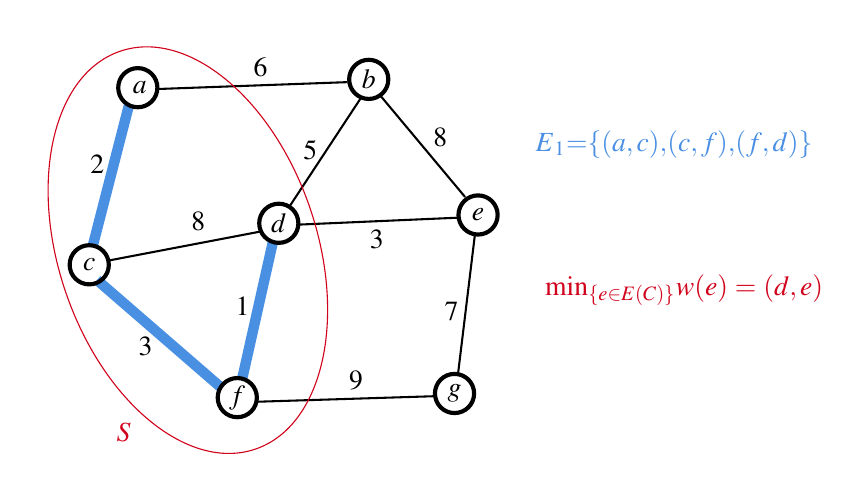
\begin{tikzpicture}[x=0.5pt,y=0.5pt,yscale=-1,xscale=1]
%uncomment if require: \path (0,332); %set diagram left start at 0, and has height of 332

%Straight Lines [id:da823970354045778] 
\draw [color={rgb, 255:red, 0; green, 0; blue, 0 }  ,draw opacity=1 ][line width=0.75]    (269,53) -- (330,126) ;
%Straight Lines [id:da271237396517352] 
\draw [color={rgb, 255:red, 0; green, 0; blue, 0 }  ,draw opacity=1 ][line width=0.75]    (179,274) -- (307,270) ;
%Straight Lines [id:da6657573604931601] 
\draw [color={rgb, 255:red, 74; green, 144; blue, 226 }  ,draw opacity=1 ][line width=3.75]    (64,186) -- (154,264) ;
%Straight Lines [id:da31661075744879486] 
\draw [color={rgb, 255:red, 0; green, 0; blue, 0 }  ,draw opacity=1 ][line width=0.75]    (72,172) -- (182,151) ;
%Straight Lines [id:da9969849240959807] 
\draw [color={rgb, 255:red, 74; green, 144; blue, 226 }  ,draw opacity=1 ][line width=3.75]    (87,60) -- (61,161) ;
%Straight Lines [id:da14506071047898028] 
\draw [color={rgb, 255:red, 0; green, 0; blue, 0 }  ,draw opacity=1 ][line width=0.75]    (107,48) -- (245,43) ;
%Straight Lines [id:da8946288202546534] 
\draw [color={rgb, 255:red, 0; green, 0; blue, 0 }  ,draw opacity=1 ][line width=0.75]    (255,54) -- (203,133) ;
%Straight Lines [id:da15496081521651384] 
\draw [color={rgb, 255:red, 74; green, 144; blue, 226 }  ,draw opacity=1 ][line width=3.75]    (191,159) -- (169,257) ;
%Straight Lines [id:da2163317830574415] 
\draw [color={rgb, 255:red, 0; green, 0; blue, 0 }  ,draw opacity=1 ][line width=0.75]    (337,154) -- (325,253) ;
%Straight Lines [id:da5391246746067021] 
\draw [color={rgb, 255:red, 0; green, 0; blue, 0 }  ,draw opacity=1 ][line width=0.75]    (324,141) -- (209,146) ;
%Shape: Ellipse [id:dp536476356315363] 
\draw  [color={rgb, 255:red, 208; green, 2; blue, 27 }  ,draw opacity=1 ] (41.23,194.4) .. controls (14.29,114.98) and (32.03,37.17) .. (80.86,20.61) .. controls (129.7,4.04) and (191.12,54.99) .. (218.07,134.41) .. controls (245.01,213.83) and (227.27,291.64) .. (178.44,308.21) .. controls (129.6,324.78) and (68.18,273.82) .. (41.23,194.4) -- cycle ;

% Text Node
\draw  [line width=1.5]   (339.38, 139) circle [x radius= 14.15, y radius= 14.15]   ;
\draw (339.38,139) node   [align=left] {$\displaystyle e$};
% Text Node
\draw  [line width=1.5]   (93.48, 47) circle [x radius= 14.15, y radius= 14.15]   ;
\draw (87.98,47) node [anchor=west] [inner sep=0.75pt]   [align=left] {$\displaystyle a$};
% Text Node
\draw  [line width=1.5]   (260.38, 41) circle [x radius= 14.15, y radius= 14.15]   ;
\draw (260.38,41) node   [align=left] {$\displaystyle b$};
% Text Node
\draw  [line width=1.5]   (58.38, 175) circle [x radius= 14.15, y radius= 14.15]   ;
\draw (58.38,175) node   [align=left] {$\displaystyle c$};
% Text Node
\draw  [line width=1.5]   (195.38, 145) circle [x radius= 14.15, y radius= 14.15]   ;
\draw (195.38,145) node   [align=left] {$\displaystyle d$};
% Text Node
\draw  [line width=1.5]   (165.38, 271) circle [x radius= 14.15, y radius= 14.15]   ;
\draw (165.38,271) node   [align=left] {$\displaystyle f$};
% Text Node
\draw  [line width=1.5]   (322.38, 268) circle [x radius= 14.15, y radius= 14.15]   ;
\draw (322.38,268) node   [align=left] {$\displaystyle g$};
% Text Node
\draw (57.24,94.06) node [anchor=north west][inner sep=0.75pt]   [align=left] {$\displaystyle 2$};
% Text Node
\draw (175.24,23.06) node [anchor=north west][inner sep=0.75pt]   [align=left] {$\displaystyle 6$};
% Text Node
\draw (259.24,148.06) node [anchor=north west][inner sep=0.75pt]   [align=left] {$\displaystyle 3$};
% Text Node
\draw (211.24,83.06) node [anchor=north west][inner sep=0.75pt]   [align=left] {$\displaystyle 5$};
% Text Node
\draw (130.24,135.06) node [anchor=north west][inner sep=0.75pt]   [align=left] {$\displaystyle 8$};
% Text Node
\draw (92.24,225.06) node [anchor=north west][inner sep=0.75pt]   [align=left] {$\displaystyle 3$};
% Text Node
\draw (162.24,196.06) node [anchor=north west][inner sep=0.75pt]   [align=left] {$\displaystyle 1$};
% Text Node
\draw (305.24,74.06) node [anchor=north west][inner sep=0.75pt]   [align=left] {$\displaystyle 8$};
% Text Node
\draw (244.24,250.06) node [anchor=north west][inner sep=0.75pt]   [align=left] {$\displaystyle 9$};
% Text Node
\draw (313.24,200) node [anchor=north west][inner sep=0.75pt]   [align=left] {$\displaystyle 7$};
% Text Node
\draw (379,76) node [anchor=north west][inner sep=0.75pt]   [align=left] {$\displaystyle \textcolor[rgb]{0.29,0.56,0.89}{E}\textcolor[rgb]{0.29,0.56,0.89}{_{1}}\textcolor[rgb]{0.29,0.56,0.89}{=}\textcolor[rgb]{0.29,0.56,0.89}{\{}\textcolor[rgb]{0.29,0.56,0.89}{(}\textcolor[rgb]{0.29,0.56,0.89}{a,c}\textcolor[rgb]{0.29,0.56,0.89}{)}\textcolor[rgb]{0.29,0.56,0.89}{,}\textcolor[rgb]{0.29,0.56,0.89}{(}\textcolor[rgb]{0.29,0.56,0.89}{c,f}\textcolor[rgb]{0.29,0.56,0.89}{)}\textcolor[rgb]{0.29,0.56,0.89}{,}\textcolor[rgb]{0.29,0.56,0.89}{(}\textcolor[rgb]{0.29,0.56,0.89}{f,d}\textcolor[rgb]{0.29,0.56,0.89}{)}\textcolor[rgb]{0.29,0.56,0.89}{\}}$};
% Text Node
\draw (76.24,287.06) node [anchor=north west][inner sep=0.75pt]   [align=left] {$\displaystyle \textcolor[rgb]{0.82,0.01,0.11}{S}$};
% Text Node
\draw (386,180) node [anchor=north west][inner sep=0.75pt]   [align=left] {$\displaystyle \textcolor[rgb]{0.82,0.01,0.11}{\min}\textcolor[rgb]{0.82,0.01,0.11}{_{\{e\in E( C)\}}}\textcolor[rgb]{0.82,0.01,0.11}{w}\textcolor[rgb]{0.82,0.01,0.11}{(}\textcolor[rgb]{0.82,0.01,0.11}{e}\textcolor[rgb]{0.82,0.01,0.11}{)}\textcolor[rgb]{0.82,0.01,0.11}{\ =\ }\textcolor[rgb]{0.82,0.01,0.11}{(}\textcolor[rgb]{0.82,0.01,0.11}{d,e}\textcolor[rgb]{0.82,0.01,0.11}{)}$};


\end{tikzpicture}

}
\caption{Illustrating the correctness of the Prim's algorithm using cut-property:
the next edge picked by the Prim's algorithm is exactly the smallest cut-edge w.r.t.\ $(S,V\setminus S)$.}
\label{fig:prim}
\end{figure}


\subsection*{Correctness of Kruskal's Algorithm}

Recall that, the Kruskal's algorithm iteratively pick the smallest edge that doesn't produce a cycle,
until $E_1$ reaches $|V| - 1$ edges. Again, at any time of the algorithm,
$E_1$ partitions all vertices into connected components $\{S_1, S_2, \cdots, S_k\}$; see Figure~\ref{fig:kruskal}.
Note that, adding an edge $e$ that doesn't produce a cycle if and only if edge $e$ spans two components~(i.e., not connect two vertices within the same component).
So, in each iteration, Kruskal's algorithm simply picks the smallest edge among these that span all pairs of
components. Without loss of generality, assume the smallest edge $e^* = (u,v)$ is between $S_i$ and $S_j$, i.e., $u\in S_i$ and $v\in S_j$.
We then define cut $C = (S_i, V\setminus S_i)$. Clearly $e^*$ is also the smallest cut-edge w.r.t.\ $C$,
because cut-edges w.r.t.\ $C$ is a subset of all ``spanning edges'' while $e^*$ is the smallest spanning edge by the algorithm.
Hence, applying the cut-property here proves that $E_1\cup \{e^*\}$ 
is a partial MST too.

\begin{figure}[h]
\centering{

\tikzset{every picture/.style={line width=0.75pt}} %set default line width to 0.75pt        

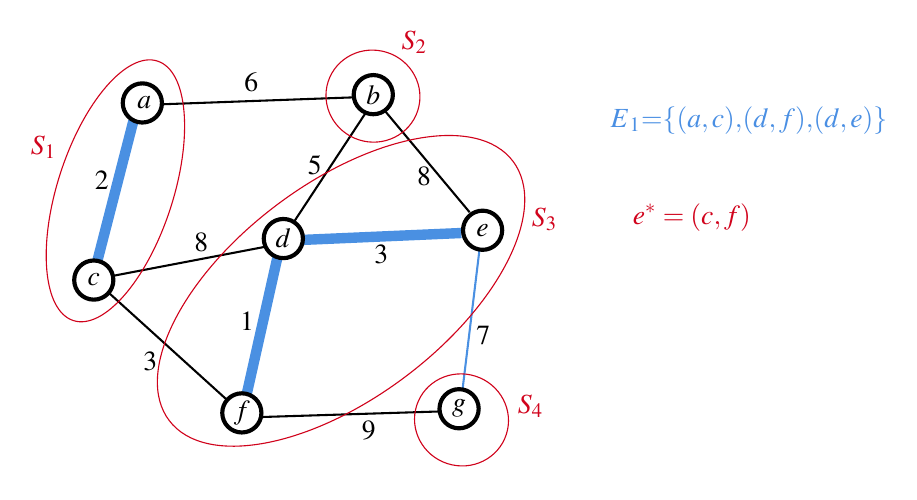
\begin{tikzpicture}[x=0.5pt,y=0.5pt,yscale=-1,xscale=1]
%uncomment if require: \path (0,371); %set diagram left start at 0, and has height of 371

%Straight Lines [id:da823970354045778] 
\draw [color={rgb, 255:red, 0; green, 0; blue, 0 }  ,draw opacity=1 ][line width=0.75]    (276,77) -- (337,150) ;
%Straight Lines [id:da271237396517352] 
\draw [color={rgb, 255:red, 0; green, 0; blue, 0 }  ,draw opacity=1 ][line width=0.75]    (186,298) -- (314,294) ;
%Straight Lines [id:da6657573604931601] 
\draw [color={rgb, 255:red, 0; green, 0; blue, 0 }  ,draw opacity=1 ][line width=0.75]    (76,208) -- (161,285) ;
%Straight Lines [id:da31661075744879486] 
\draw [color={rgb, 255:red, 0; green, 0; blue, 0 }  ,draw opacity=1 ][line width=0.75]    (79,196) -- (189,175) ;
%Straight Lines [id:da9969849240959807] 
\draw [color={rgb, 255:red, 74; green, 144; blue, 226 }  ,draw opacity=1 ][line width=3.75]    (94,84) -- (68,185) ;
%Straight Lines [id:da14506071047898028] 
\draw [color={rgb, 255:red, 0; green, 0; blue, 0 }  ,draw opacity=1 ][line width=0.75]    (114,72) -- (252,67) ;
%Straight Lines [id:da8946288202546534] 
\draw [color={rgb, 255:red, 0; green, 0; blue, 0 }  ,draw opacity=1 ][line width=0.75]    (262,78) -- (210,157) ;
%Straight Lines [id:da15496081521651384] 
\draw [color={rgb, 255:red, 74; green, 144; blue, 226 }  ,draw opacity=1 ][line width=3.75]    (198,183) -- (176,281) ;
%Straight Lines [id:da2163317830574415] 
\draw [color={rgb, 255:red, 74; green, 144; blue, 226 }  ,draw opacity=1 ][line width=0.75]    (344,178) -- (332,277) ;
%Straight Lines [id:da5391246746067021] 
\draw [color={rgb, 255:red, 74; green, 144; blue, 226 }  ,draw opacity=1 ][line width=3.75]    (331,165) -- (216,170) ;
%Shape: Ellipse [id:dp8079044569602617] 
\draw  [color={rgb, 255:red, 208; green, 2; blue, 27 }  ,draw opacity=1 ] (41.31,121.62) .. controls (58.12,69.84) and (89.51,33.63) .. (111.43,40.74) .. controls (133.35,47.86) and (137.49,95.6) .. (120.69,147.38) .. controls (103.88,199.16) and (72.49,235.37) .. (50.57,228.26) .. controls (28.65,221.14) and (24.51,173.4) .. (41.31,121.62) -- cycle ;
%Shape: Ellipse [id:dp9738354187366457] 
\draw  [color={rgb, 255:red, 208; green, 2; blue, 27 }  ,draw opacity=1 ] (197.42,144.88) .. controls (266.03,93.16) and (342.55,78.94) .. (368.33,113.13) .. controls (394.1,147.32) and (359.37,216.97) .. (290.75,268.7) .. controls (222.13,320.42) and (145.61,334.64) .. (119.84,300.45) .. controls (94.07,266.26) and (128.8,196.61) .. (197.42,144.88) -- cycle ;
%Shape: Ellipse [id:dp2276168529447603] 
\draw  [color={rgb, 255:red, 208; green, 2; blue, 27 }  ,draw opacity=1 ] (234.76,55.56) .. controls (240.41,38.13) and (259.49,28.7) .. (277.37,34.51) .. controls (295.25,40.31) and (305.16,59.14) .. (299.5,76.57) .. controls (293.85,94.01) and (274.77,103.43) .. (256.89,97.63) .. controls (239.01,91.83) and (229.1,72.99) .. (234.76,55.56) -- cycle ;
%Shape: Ellipse [id:dp3153590720909477] 
\draw  [color={rgb, 255:red, 208; green, 2; blue, 27 }  ,draw opacity=1 ] (298.76,289.56) .. controls (304.41,272.13) and (323.49,262.7) .. (341.37,268.51) .. controls (359.25,274.31) and (369.16,293.14) .. (363.5,310.57) .. controls (357.85,328.01) and (338.77,337.43) .. (320.89,331.63) .. controls (303.01,325.83) and (293.1,306.99) .. (298.76,289.56) -- cycle ;

% Text Node
\draw  [line width=1.5]   (346.38, 163) circle [x radius= 14.15, y radius= 14.15]   ;
\draw (346.38,163) node   [align=left] {$\displaystyle e$};
% Text Node
\draw  [line width=1.5]   (100.48, 71) circle [x radius= 14.15, y radius= 14.15]   ;
\draw (94.98,71) node [anchor=west] [inner sep=0.75pt]   [align=left] {$\displaystyle a$};
% Text Node
\draw  [line width=1.5]   (267.38, 65) circle [x radius= 14.15, y radius= 14.15]   ;
\draw (267.38,65) node   [align=left] {$\displaystyle b$};
% Text Node
\draw  [line width=1.5]   (65.38, 199) circle [x radius= 14.15, y radius= 14.15]   ;
\draw (65.38,199) node   [align=left] {$\displaystyle c$};
% Text Node
\draw  [line width=1.5]   (202.38, 169) circle [x radius= 14.15, y radius= 14.15]   ;
\draw (202.38,169) node   [align=left] {$\displaystyle d$};
% Text Node
\draw  [line width=1.5]   (172.38, 295) circle [x radius= 14.15, y radius= 14.15]   ;
\draw (172.38,295) node   [align=left] {$\displaystyle f$};
% Text Node
\draw  [line width=1.5]   (329.38, 292) circle [x radius= 14.15, y radius= 14.15]   ;
\draw (329.38,292) node   [align=left] {$\displaystyle g$};
% Text Node
\draw (64.24,118.06) node [anchor=north west][inner sep=0.75pt]   [align=left] {$\displaystyle 2$};
% Text Node
\draw (172.24,47.06) node [anchor=north west][inner sep=0.75pt]   [align=left] {$\displaystyle 6$};
% Text Node
\draw (266.24,172.06) node [anchor=north west][inner sep=0.75pt]   [align=left] {$\displaystyle 3$};
% Text Node
\draw (218.24,107.06) node [anchor=north west][inner sep=0.75pt]   [align=left] {$\displaystyle 5$};
% Text Node
\draw (136.24,163.06) node [anchor=north west][inner sep=0.75pt]   [align=left] {$\displaystyle 8$};
% Text Node
\draw (99.24,249.06) node [anchor=north west][inner sep=0.75pt]   [align=left] {$\displaystyle 3$};
% Text Node
\draw (169.24,220.06) node [anchor=north west][inner sep=0.75pt]   [align=left] {$\displaystyle 1$};
% Text Node
\draw (297.24,115.06) node [anchor=north west][inner sep=0.75pt]   [align=left] {$\displaystyle 8$};
% Text Node
\draw (257.24,299.06) node [anchor=north west][inner sep=0.75pt]   [align=left] {$\displaystyle 9$};
% Text Node
\draw (340,230.5) node [anchor=north west][inner sep=0.75pt]   [align=left] {$\displaystyle 7$};
% Text Node
\draw (437,72) node [anchor=north west][inner sep=0.75pt]   [align=left] {$\displaystyle \textcolor[rgb]{0.29,0.56,0.89}{E}\textcolor[rgb]{0.29,0.56,0.89}{_{1}}\textcolor[rgb]{0.29,0.56,0.89}{=}\textcolor[rgb]{0.29,0.56,0.89}{\{}\textcolor[rgb]{0.29,0.56,0.89}{(}\textcolor[rgb]{0.29,0.56,0.89}{a,c}\textcolor[rgb]{0.29,0.56,0.89}{)}\textcolor[rgb]{0.29,0.56,0.89}{,}\textcolor[rgb]{0.29,0.56,0.89}{(}\textcolor[rgb]{0.29,0.56,0.89}{d,f}\textcolor[rgb]{0.29,0.56,0.89}{)}\textcolor[rgb]{0.29,0.56,0.89}{,}\textcolor[rgb]{0.29,0.56,0.89}{(}\textcolor[rgb]{0.29,0.56,0.89}{d,e}\textcolor[rgb]{0.29,0.56,0.89}{)}\textcolor[rgb]{0.29,0.56,0.89}{\}}$};
% Text Node
\draw (18,93) node [anchor=north west][inner sep=0.75pt]   [align=left] {$\displaystyle \textcolor[rgb]{0.82,0.01,0.11}{S}\textcolor[rgb]{0.82,0.01,0.11}{_{1}}$};
% Text Node
\draw (286,17) node [anchor=north west][inner sep=0.75pt]   [align=left] {$\displaystyle \textcolor[rgb]{0.82,0.01,0.11}{S}\textcolor[rgb]{0.82,0.01,0.11}{_{2}}$};
% Text Node
\draw (380,145) node [anchor=north west][inner sep=0.75pt]   [align=left] {$\displaystyle \textcolor[rgb]{0.82,0.01,0.11}{S}\textcolor[rgb]{0.82,0.01,0.11}{_{3}}$};
% Text Node
\draw (370,280) node [anchor=north west][inner sep=0.75pt]   [align=left] {$\displaystyle \textcolor[rgb]{0.82,0.01,0.11}{S}\textcolor[rgb]{0.82,0.01,0.11}{_{4}}$};
% Text Node
\draw (453,142) node [anchor=north west][inner sep=0.75pt]   [align=left] {$\displaystyle \textcolor[rgb]{0.82,0.01,0.11}{e^{*} =( c,f)}$};


\end{tikzpicture}

}
\caption{Illustrating the correctness of the Kruskal's algorithm using cut-property:
the smallest spanning edge $e^*$ picked by the algorithm is also the smallest cut-edge
	w.r.t.\ cut $(S_i,V\setminus S_i)$ where $S_i = S_1$~(or $S_i = S_2$).  }
\label{fig:kruskal}
\end{figure}


\end{document}
